\newthought{\textbf{M.IKHSAN - 2020903430016 - TRKJ 3B}}

\newday{\textbf{01 Desember 2022}}
\begin{enumerate}
\item Kendala
% jelaskan kendala dan penyebab yang dialami saat mengikuti praktikum serta solusi atau langkah-langkah yang telah dilakukan
\newline 
sudah berhasil menginstall hadoop

\item solusi
\newline
menginstal ulang ubuntu

\item Kesimpulan
% berikan kesimpulan dari praktikum yang telah dikerjkan
\newline
setelah menginstall ulang ubuntu, instalasi dan konfigurasi hadoop berhasil

\begin{figure}[!ht]
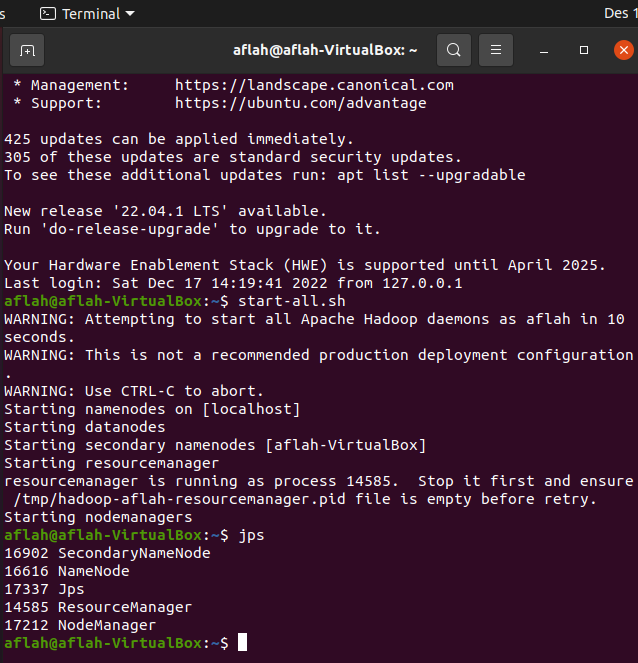
\includegraphics[width=\textwidth]{M.IKHSAN/jps}
\caption{Verifikasi Hasil Instalasi Hadoop}
\label{gam:Java-version(M.IKHSAN)}
\end{figure} 

\begin{figure}[!ht]
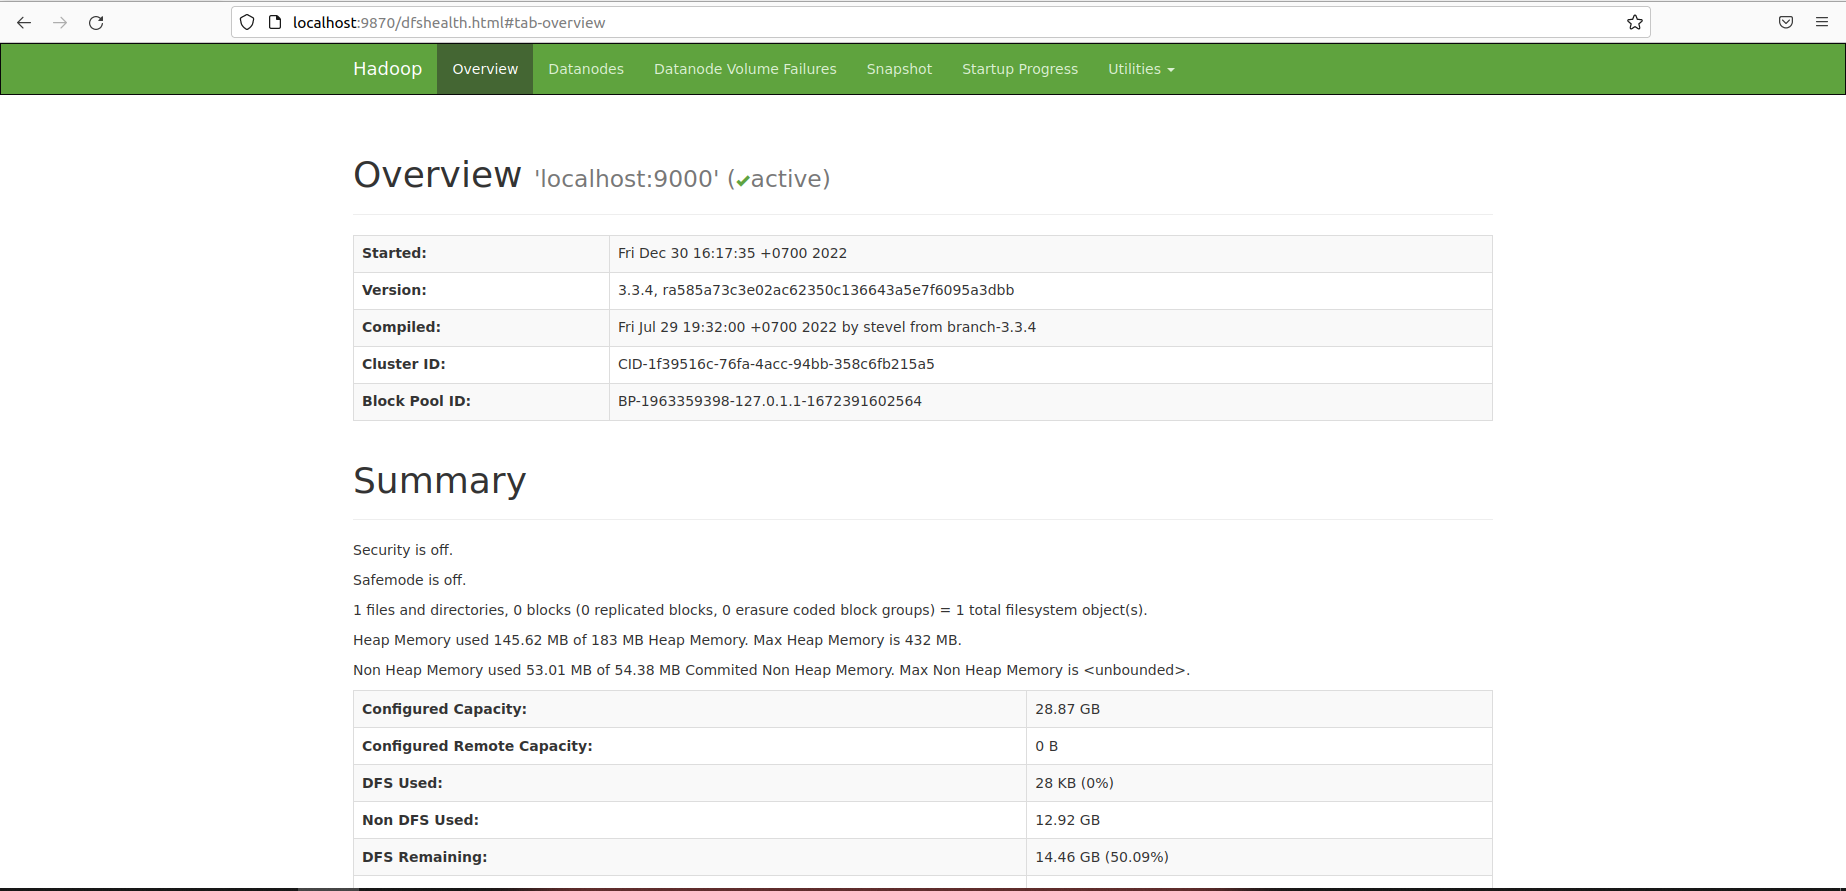
\includegraphics[width=\textwidth]{M.IKHSAN/localhost1}
\caption{Verifikasi Hasil Instalasi Hadoop}
\label{gam:Java-version(M.IKHSAN)}
\end{figure} 

\begin{figure}[!ht]
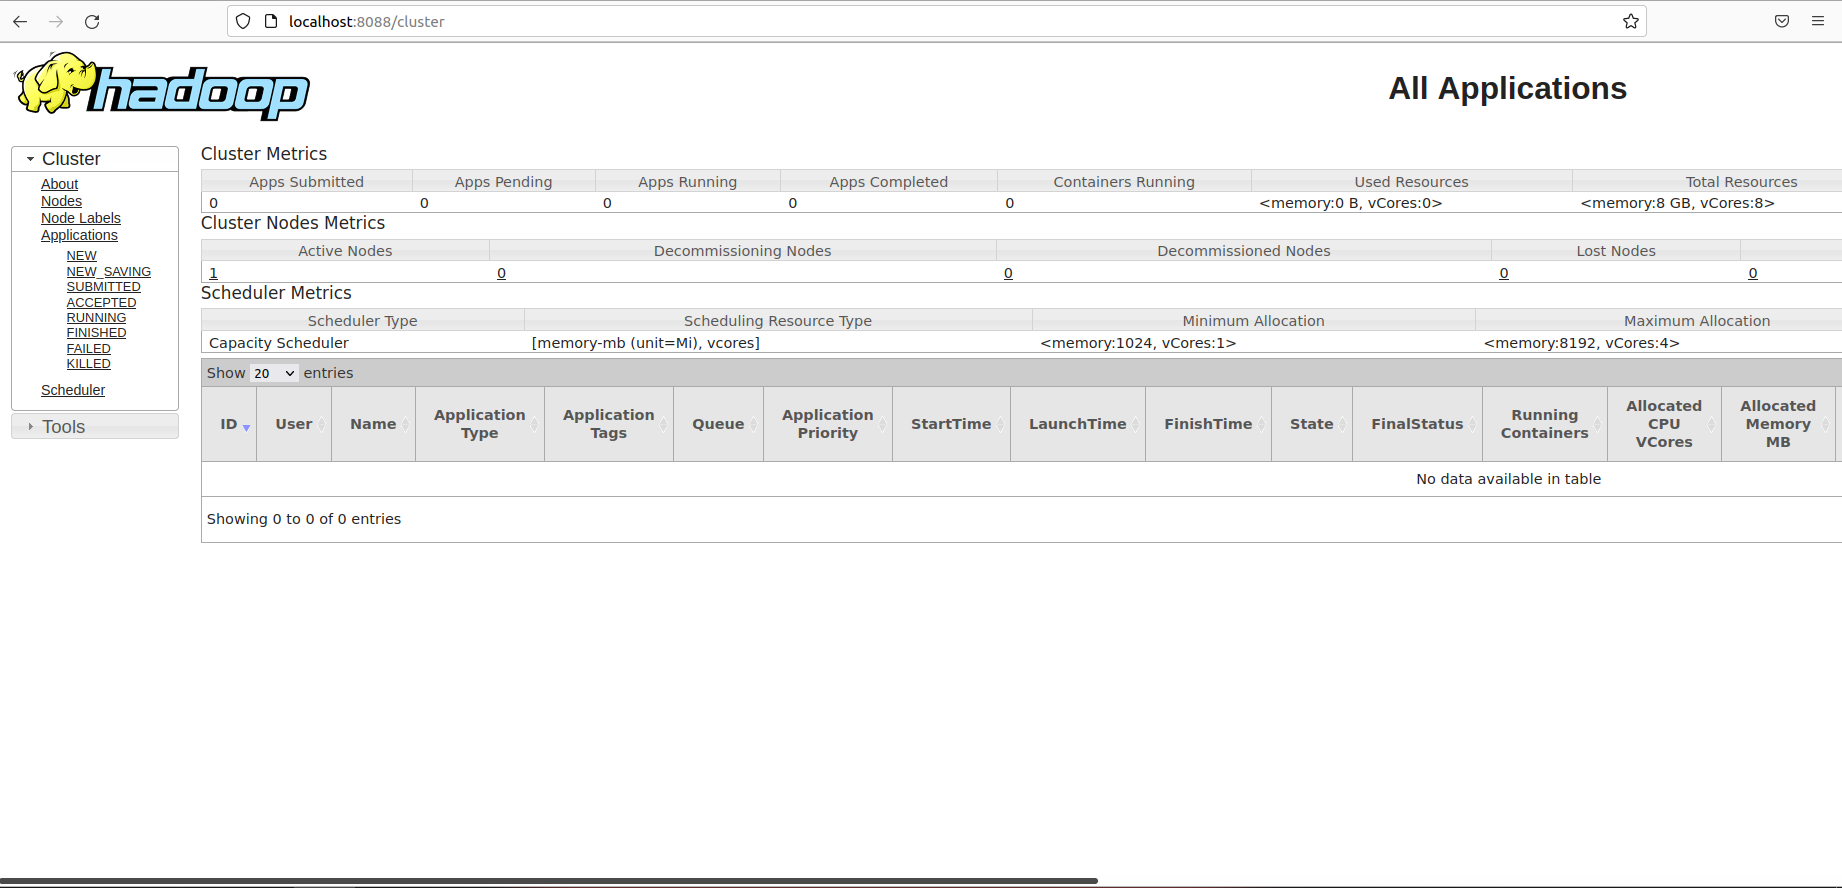
\includegraphics[width=\textwidth]{M.IKHSAN/localhost2}
\caption{Verifikasi Hasil Instalasi Hadoop}
\label{gam:Hadoop-version(M.IKHSAN)}
\end{figure}

\end{enumerate}


\newday{\textbf{02 Desember 2022}}
\begin{enumerate}
\item Kendala dan Solusi
% jelaskan kendala dan penyebab yang dialami saat mengikuti praktikum serta solusi atau langkah-langkah yang telah dilakukan

\item Kesimpulan
% berikan kesimpulan dari praktikum yang telah dikerjkan

\end{enumerate}

\newday{\textbf{08 Desember 2022}}
\begin{enumerate}
\item Kendala dan Solusi
% jelaskan kendala dan penyebab yang dialami saat mengikuti praktikum serta solusi atau langkah-langkah yang telah dilakukan

\item Kesimpulan
% berikan kesimpulan dari praktikum yang telah dikerjkan

\end{enumerate}


\newday{\textbf{09 Desember 2022}}
\begin{enumerate}
\item Kendala dan Solusi
% jelaskan kendala dan penyebab yang dialami saat mengikuti praktikum serta solusi atau langkah-langkah yang telah dilakukan


\item Kesimpulan
% berikan kesimpulan dari praktikum yang telah dikerjkan

\end{enumerate}

\newday{\textbf{15 Desember 2022}}
\begin{enumerate}
\item Kendala dan Solusi
\newline pada praktikum kali ini membuat program WordCount Bawaan Hadoop. pada saat praktikum tidak ada kendala hanya saja error karena salah menulis perintah.

\item Kesimpulan
Berhasil mencoba program bawaan Hadoop yaitu program menghitung jumlah kata dalam data input yang diberikan. Berikut ini gambar bukti keberhasilan praktikum.

\begin{figure}[!ht]
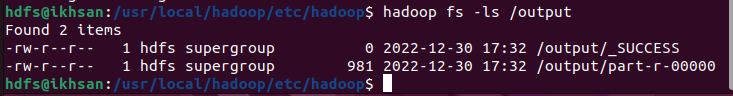
\includegraphics[width=\textwidth]{M.IKHSAN/wordcount bawaan1}
\caption{Cek Hasil}
\label{gam:Hadoop-version(M.IKHSAN)}
\end{figure}

\begin{figure}[!ht]
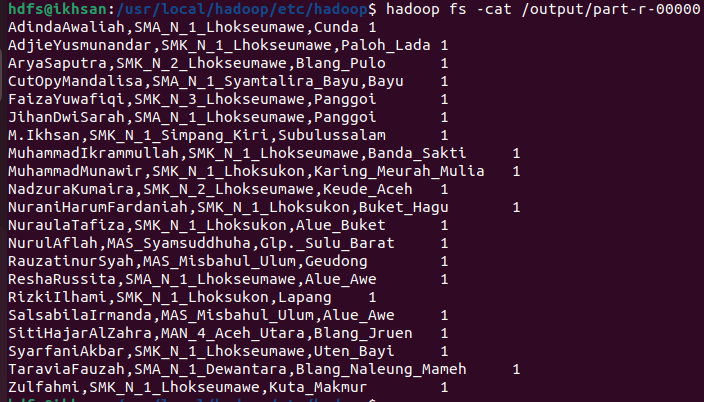
\includegraphics[width=\textwidth]{M.IKHSAN/WordCount}
\caption{Lihat Hasil}
\label{gam:Hadoop-version(M.IKHSAN)}
\end{figure}
\begin{figure}[!ht]
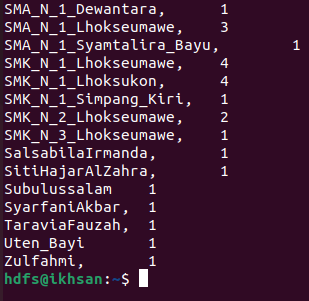
\includegraphics[width=\textwidth]{M.IKHSAN/WordCount2}
\caption{Lihat Hasil}
\label{gam:Hadoop-version(M.IKHSAN)}
\end{figure}
\end{enumerate}

\clearpage
\newday{\textbf{16 Desember 2022}}
\begin{enumerate}
\item Kendala
terdapat error pada perintah 6 dan 7

\item Solusi
- pada perintah no 6 saya memberi spasi antara JavaCompiled/ dengan WordCount.Java
- pada perintah no 7 saya kurang teliti di bagian JavaCompiled/ .


\item Kesimpulan
Untuk hasil yang ditampikan sama dengan WordCount bawaan hadoop.

\begin{figure}[!ht]
    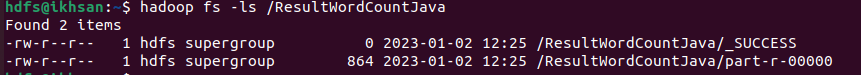
\includegraphics[width=\textwidth]{M.IKHSAN/WordCount java.PNG}
    \caption{hasil WordCount Java }
    \label{gam:hasil}
    \end{figure}
\begin{figure}[!ht]
    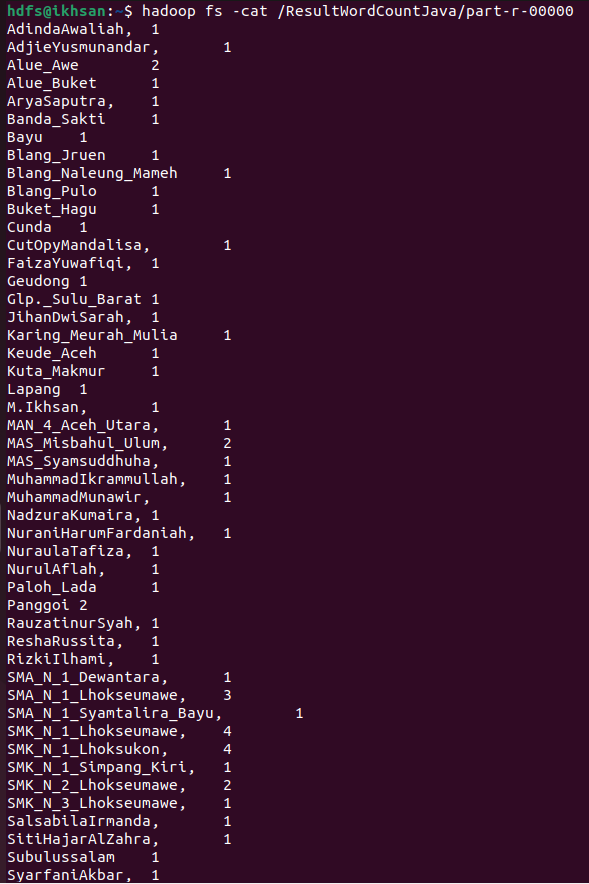
\includegraphics[width=\textwidth]{M.IKHSAN/WordCount java1.PNG}
    \caption{hasil WordCount Java }
    \label{gam:hasil}
    \end{figure}
\begin{figure}[!ht]
    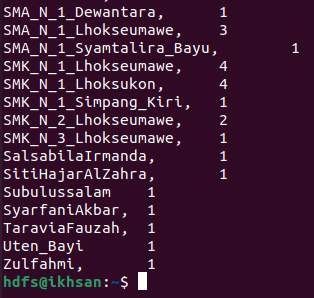
\includegraphics[width=\textwidth]{M.IKHSAN/WordCount java2.PNG}
    \caption{hasil WordCount Java}
    \label{gam:hasil}
    \end{figure}
\end{enumerate}

\newday{\textbf{22 Desember 2022}}
\begin{enumerate}
\item Kendala dan Solusi
% jelaskan kendala dan penyebab yang dialami saat mengikuti praktikum serta solusi atau langkah-langkah yang telah dilakukan

\begin{itemize}
\item Tidak menemukan masalah apapun
\end{itemize}

\item Kesimpulan
\newline
Apache Spark adalah sebuah framework komputasi yang dapat digunakan untuk mengakses data, memproses data, menanyakan data serta menganalisis big data

\begin{figure}[!ht]
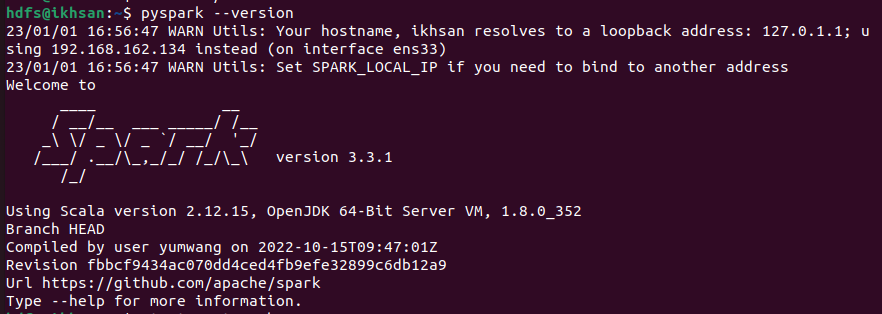
\includegraphics[width=\textwidth]{M.IKHSAN/SPARK}
\caption{hasil instalasi apache spark }
\label{gam:hasil instalasi spark}
\end{figure}
\end{enumerate}

\newday{\textbf{23 Desember 2022}}
\begin{enumerate}
\item Kendala dan Solusi
% jelaskan kendala dan penyebab yang dialami saat mengikuti praktikum serta solusi atau langkah-langkah yang telah dilakukan

\item Kesimpulan
% berikan kesimpulan dari praktikum yang telah dikerjkan

\end{enumerate}

\newday{\textbf{02 Januari 2023} Wordcountpyspark}
\begin{enumerate}
\item Kendala dan Solusi
\item tidak menemukan masalah pada pratikum

\item Kesimpulan
Berhasil menjalankan program menggunakan PySpark

\begin{figure}[!ht]
    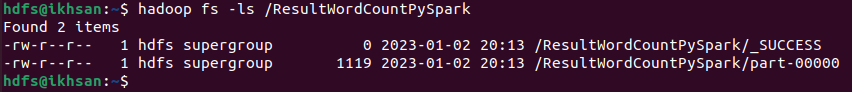
\includegraphics[width=\textwidth]{M.IKHSAN/wordcountpyspark}
    \caption{hasil program WordCountPySpark }
    \label{gam:hasil instalasi spark}
    \end{figure}
\begin{figure}[!ht]
    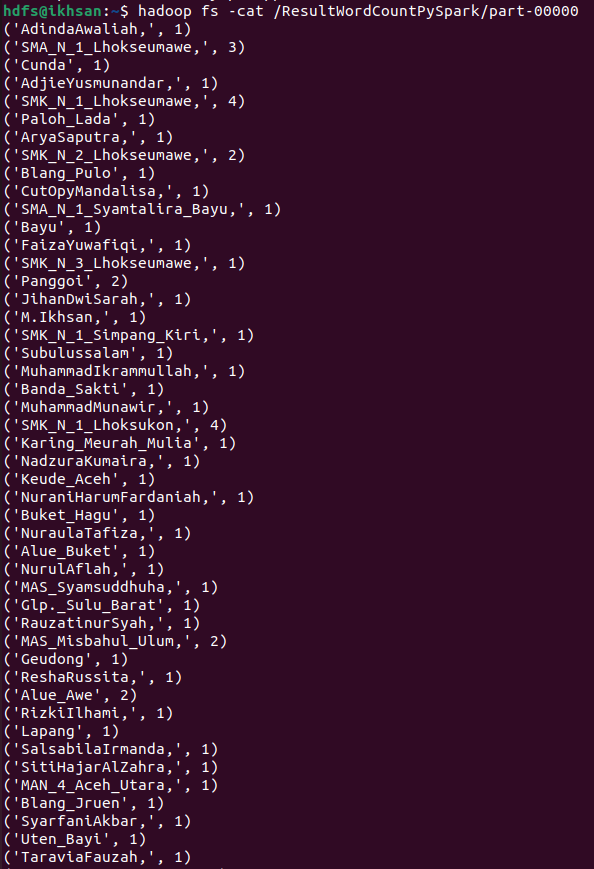
\includegraphics[width=\textwidth]{M.IKHSAN/wordcountpyspark1}
    \caption{hasil program WordCountPySpark }
    \label{gam:hasil instalasi spark}
    \end{figure}
\begin{figure}[!ht]
    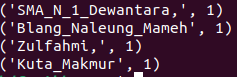
\includegraphics[width=\textwidth]{M.IKHSAN/wordcountpyspark2}
    \caption{hasil program WordCountPySpark }
    \label{gam:hasil instalasi spark}
    \end{figure}
\end{enumerate}